\documentclass[12pt,a4paper]{article}
\usepackage[utf8]{inputenc}
\usepackage{geometry}
\usepackage{titlesec} % For customizing section titles
\usepackage{graphicx} % For images
\usepackage{hyperref} % For hyperlinks
\usepackage{fancyhdr} % For fancy headers and footers
\usepackage{lipsum} % For generating dummy text
\usepackage{graphicx}
\usepackage{subcaption}
\usepackage{dirtree}

% Set page geometry
\geometry{left=2.5cm, right=2.5cm, top=2.5cm, bottom=2.5cm}

% Set up hyperref
\hypersetup{
    colorlinks=true,
    allcolors=blue,
    linkcolor=black,
    filecolor=cyan,
    urlcolor=blue,
}

% Customize section titles
\titleformat{\section}{\large\bfseries}{\thesection}{1em}{}
\titleformat{\subsection}{\normalsize\bfseries}{\thesubsection}{1em}{}

% Setup headers and footers
\pagestyle{fancy}
\fancyhf{}
\rhead{3D printing defect detection}
\lhead{Data provisioning}
\rfoot{Page \thepage}

% Title and author
\title{{\textbf{Data provisioning for 3D printing defect (spaghetti) detection}\\ {\small Full version}}}
\author{Michal Raczkowski}
\date{15-01-2024}

\begin{document}

\maketitle
\thispagestyle{empty} % Remove header/footer for the first page

% Insert table of contents
\newpage
\tableofcontents
\newpage

\setcounter{page}{1} % Start page numbering from here

\section{Introduction}
This document outlines the process of data collection, processing, and labeling for training a YOLO algorithm in detecting defects in 3D printing, with a focus on the "spaghetti" issue.

\section{Data Requirements}
YOLO algorithm require set of labeled images in YOLO format representing the object we wish the algorithm to recognize. Those images have to be free to use.

\section{Data Collection}
Data is collected from homemade pictures displaying failing prints with certain defect and from online open sources\cite{onlineOpenSource1},\cite{onlineOpenSource2}.

\section{Data Understanding}
Because datasets are made out of photos which displays various types of 3D printed defects we have to choose images which displays relevant issue (spaghetti defect) to our use case
\begin{figure}[h]
    \centering
    \begin{subfigure}[b]{0.45\textwidth}
        \centering
        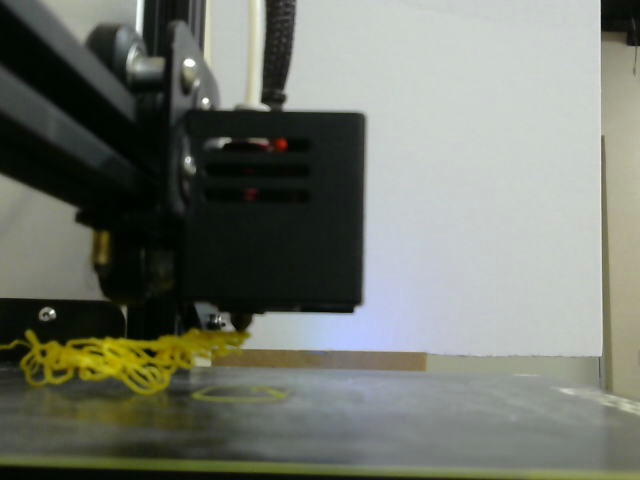
\includegraphics[width=\textwidth]{no_support_0.jpg}
        \caption{"Spaghetti" issue\cite{onlineOpenSource1}}
        \label{fig:image1}
    \end{subfigure}
    \begin{subfigure}[b]{0.45\textwidth}
        \centering
        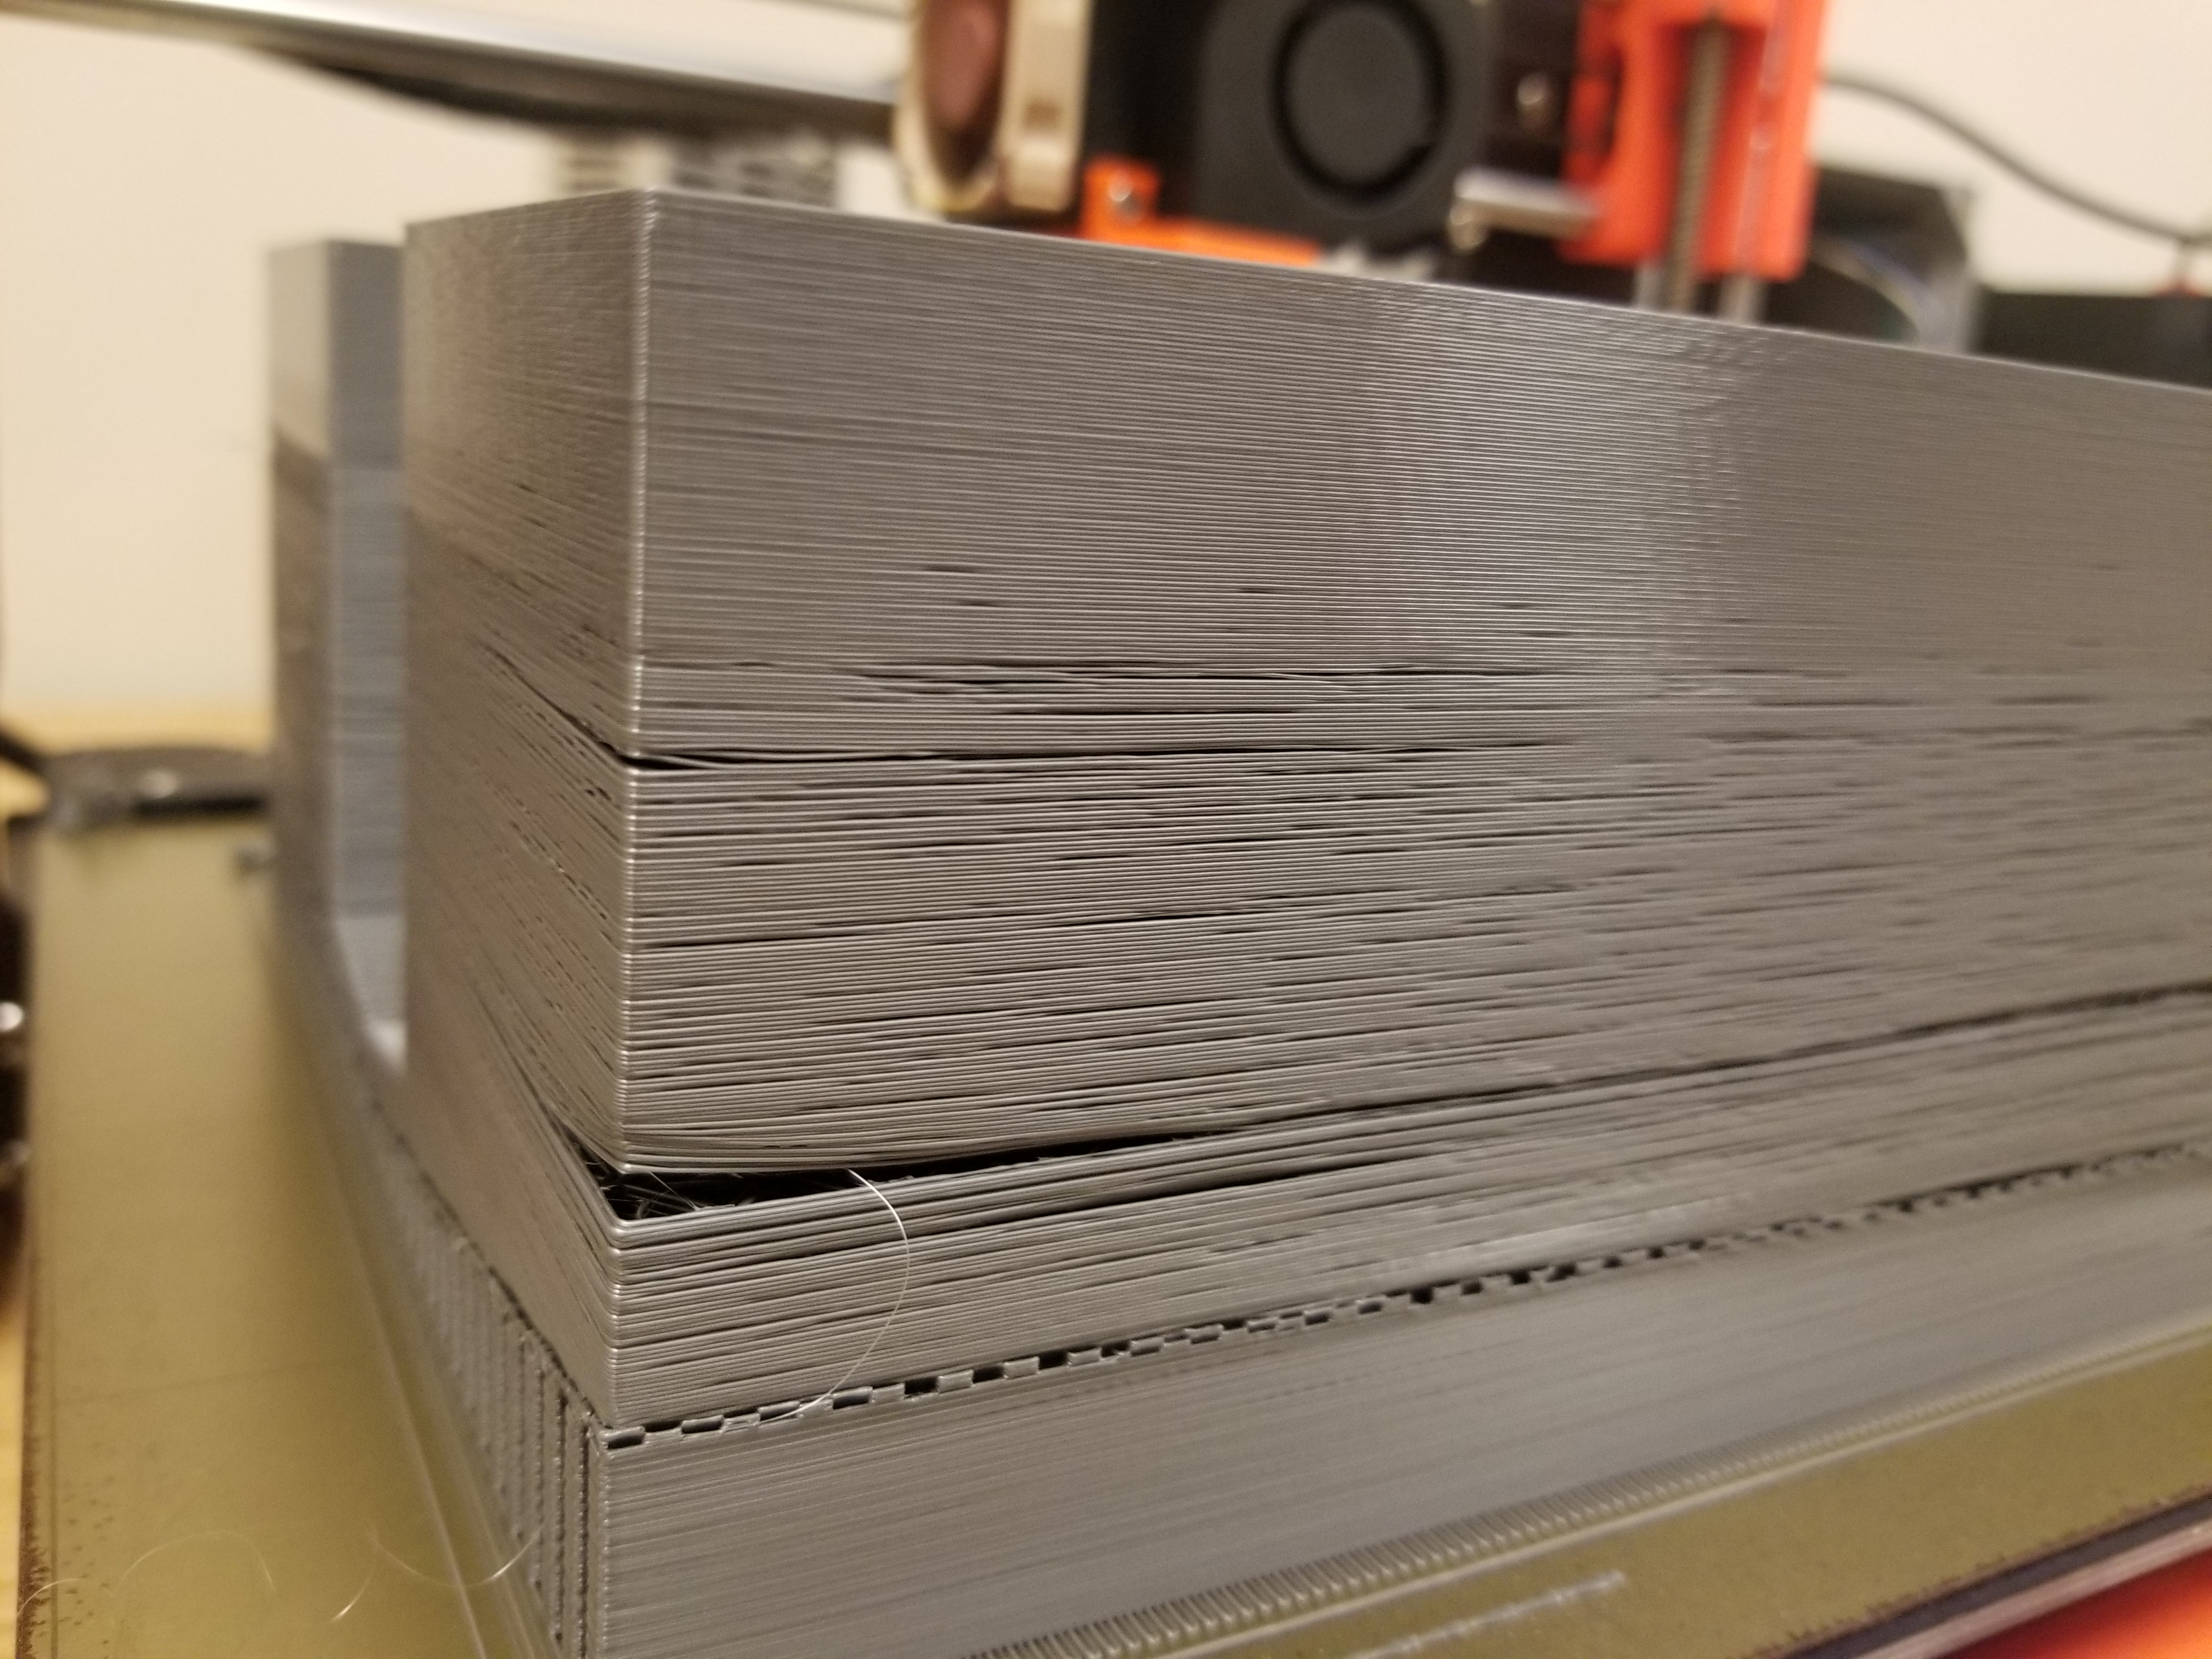
\includegraphics[width=\textwidth]{24382-129778-20190220-061954.jpg}
        \caption{Layers split issue\cite{onlineOpenSource2}}
        \label{fig:image2}
    \end{subfigure}
    \hfill

    \caption{Two types of 3D printing issues}
    \label{fig:test}
\end{figure}
\\In example images above we can see two types of 3d printing issues.

\begin{itemize}
    \item Figure \ref{fig:image1} we can see issue we are interested in which is "spaghetti" issue it characterize by disorganized, tangled layers of filament, resembling spaghetti, resulting from print errors. 
    \item Figure \ref{fig:image2} we can see issue which we are not interested because it doesn't display "spaghetti" issue which we are focusing on, it displays layers split issue which characterize by distinct gaps and separations between layers, compromising print integrity and appearance
\end{itemize}

From looking on pictures and understanding displayed issues we can come to conclusion that Figure \ref{fig:image1} will be relevant to our dataset, because it displays "spaghetti" issue which we are focusing on. This kind of filtering have to be done by hand, or we can try to find dataset containing already described images.
\section{Data Processing}
\subsection{Dataset structure}
Dataset we are using is composed of main two important parts:
\begin{itemize}
    \item \textbf{Images}: Display issue of our interest (spaghetti issue)
    
    \item \textbf{Labels}: Set of annotations on an image that define the location (through bounding box coordinates) and type (class information) of each object within the image. 
\end{itemize}
For better understanding here is structure of directories:
\smallbreak
{\dirtree{%
.1 data/.
.2 images/.
.3 train/.
.4 ....
.3 val/.
.4 ....
.2 labels/.
.4 ....
.3 train/.
.4 ....
.3 val/.
}}
\medbreak
\noindent
Directories \verb|train| contains data on which model is trained 
\smallbreak
\noindent
Directories \verb|val| contains data on which model is validated 
\subsection{Why we need to add labels to images?}

Labeling images is essential in training the YOLO (You Only Look Once) object detection algorithm for several reasons: 

\begin{itemize}
    \item \textbf{Training Supervision}: Labels provide the algorithm with examples to learn from, indicating what objects are present in the image and where they are.
    \item \textbf{Bounding Box Coordinates}:Labels include bounding box coordinates to teach the model how to locate and size objects in an image. 
    \item \textbf{Class Identification}: Labels assign a class to each object, helping the model to classify objects correctly.
    \item  \textbf{Model Accuracy and Evaluation}: Good quality labels improve the accuracy of the model and allow for effective evaluation of its performance.
    \item \textbf{Algorithm Optimization}:Accurate labels are crucial for minimizing the loss during training and optimizing the algorithm's performance.
\end{itemize}
\newpage

\subsection{Process of labeling}
 There are various tools we can use to label data (e.g. CVAT{ \scriptsize \cite{labelingTool1}}, VoTT{ \scriptsize \cite{labelingTool2}}) but to keep simplicity and be able of rapid prototyping we are using free open source online tool called {\textbf {MakeSense}}{ \scriptsize \cite{labelingTool3}} which is capable enough for our purposes 
 \begin{figure}[h]
    \centering
    \begin{subfigure}[b]{0.45\textwidth}
        \centering
        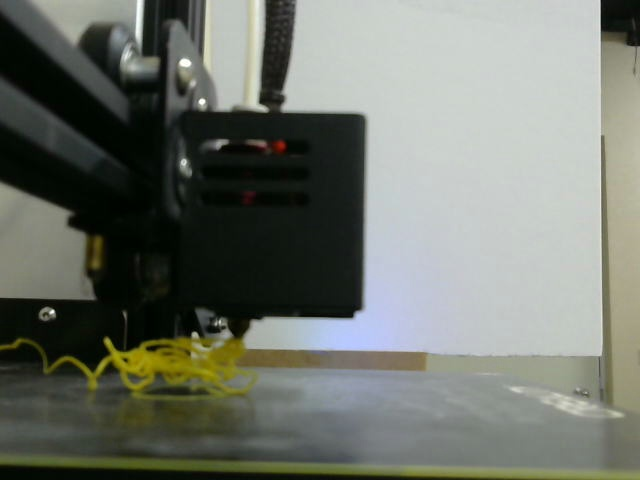
\includegraphics[width=\textwidth]{no_support_62.jpg}
        \caption{no\_support\_62.jpeg \cite{onlineOpenSource2}}
        \label{fig:image1}
    \end{subfigure}
    \begin{subfigure}[b]{0.45\textwidth}
        \centering
        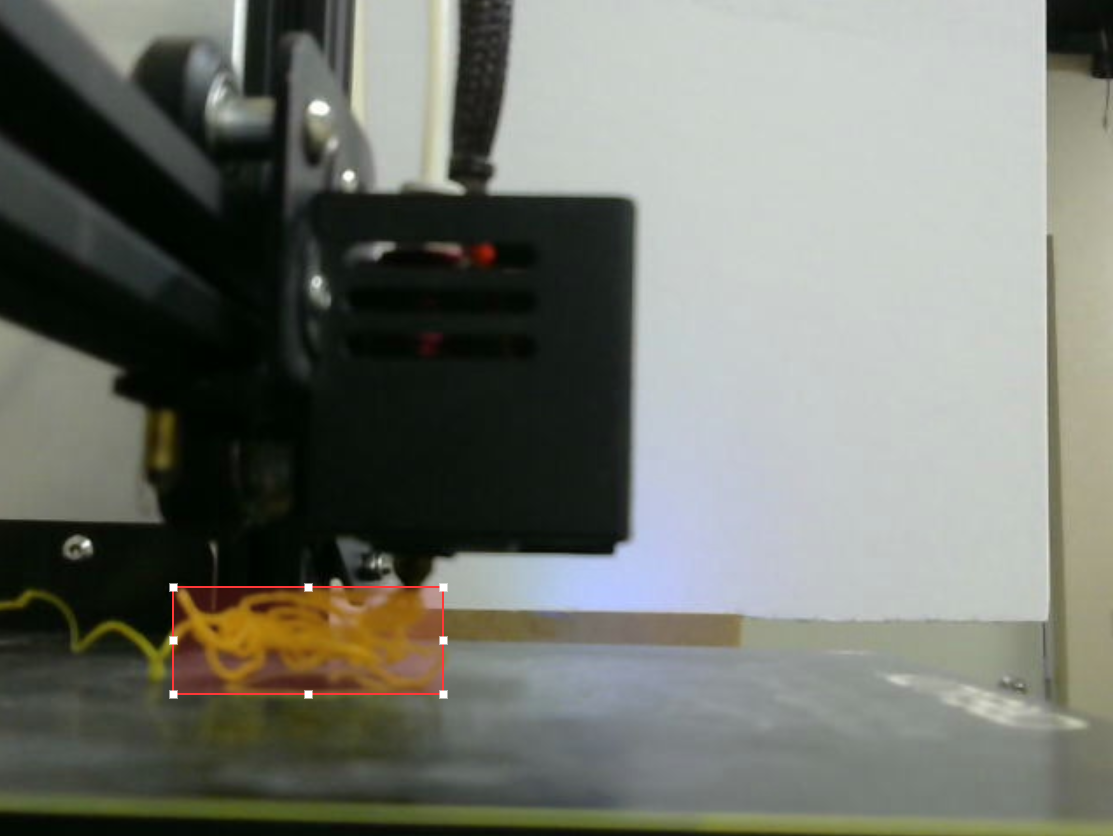
\includegraphics[width=\textwidth]{LabelByMakeSens.png}
        \caption{no\_support\_62.jpeg (labeled)\cite{onlineOpenSource2}}
        \label{fig:image2}
    \end{subfigure}
    \hfill

    \caption{Comparison of image without and with label}
    \label{fig:test}
\end{figure}
\\Labeling involves identifying and marking the coordinates on an image to pinpoint the location of the defect we aim to detect in our case "spaghetti" defect. Once we have labeled all the images, we can export our labels in the YOLO format, which is specifically designed for the YOLO algorithm. 
\subsection{Dataset final structure}

The final dataset should have this directory structure:
{\dirtree{%
.1 data/.
.2 images/.
.3 train/.
.4 no\_support\_62.jpeg .
.4 ....
.3 val/.
.4 exampleValidationImage.jpeg .
.4 ....
.2 labels/.
.3 train/.
.4 no\_support\_62.txt .
.4 ....
.3 val/.
.4 exampleValidationImage.txt .
.4 ....
}}
We can observe that labels are stored in separate directories, yet they share the same names as their corresponding images. This correlation is essential, as it enables the algorithm to accurately pair each image file with its respective label file. Additionally, it's important to note that the final dataset will contain many images along with their corresponding labels.
\newpage

\subsection{Label explained}
\noindent
Here is an example of what the contents of a label file might look like: \smallbreak
\verb|0 0.281250 0.764286 0.244643 0.130952| \smallbreak
\noindent
The meaning of sentence above is as follows: 
\begin{itemize}
    \item \verb|0|: number of a class
    \item \verb|0.281250|: X coordinate of center of the box
    \item \verb|0.764286|: Y coordinate of center of the box
    \item \verb|0.244643|: width of the box
    \item \verb|0.130952|: height of the box
\end{itemize}

\section{Conclusion}
After preforming all those task and reading about importance of labeling in YOLO algorithm we should be capable to prepare our own dataset for YOLO algorithm to detect "spaghetti" issue in 3D printing


\begin{thebibliography}{9}

    \bibitem{onlineOpenSource1}
        Dataset: \href{https://www.kaggle.com/datasets/justin900429/3d-printer-defected-dataset}{3D-Printer Defected Dataset}: \\
        {\footnotesize \url{https://www.kaggle.com/datasets/justin900429/3d-printer-defected-dataset}}
    \bibitem{onlineOpenSource2}
        Dataset: \href{https://www.kaggle.com/datasets/mikulhe/3d-printing-errors}{3D printing errors}: \\
        {\footnotesize \url{https://www.kaggle.com/datasets/mikulhe/3d-printing-errors}}
    \bibitem{labelingTool1}
        Computer Vision Annotation Tool: \href{https://www.cvat.ai/}{CVAT}: \\
        {\footnotesize \url{https://www.cvat.ai/}}
    \bibitem{labelingTool2}
        Visual Object Tagging Tool: \href{https://github.com/microsoft/VoTT}{VoTT}: \\
        {\footnotesize \url{https://github.com/microsoft/VoTT}}
    \bibitem{labelingTool3}
        MakeSense: \href{https://www.makesense.ai/}{MakeSense}: \\
        {\footnotesize \url{https://www.makesense.ai/}}

    \end{thebibliography}

\end{document}
